\chapter{ANALYSE ET CONCEPTION GENERALE}


Nous allons dans ce chapitre présenté le modèle d’analyse qui sera utilisé dans notre application et la conception.

\section{ANALYSE} 

\subsection{DIAGRAMME DE CAS D’UTILISATION}
C’est un des diagrammes UML utilisés pour donner une vision globale du comportement fonctionnel d'un système logiciel. Un cas d'utilisation représente une unité discrète d'interaction entre un utilisateur (humain ou machine) et un système


\begin{figure}[h]
	\begin{center}
		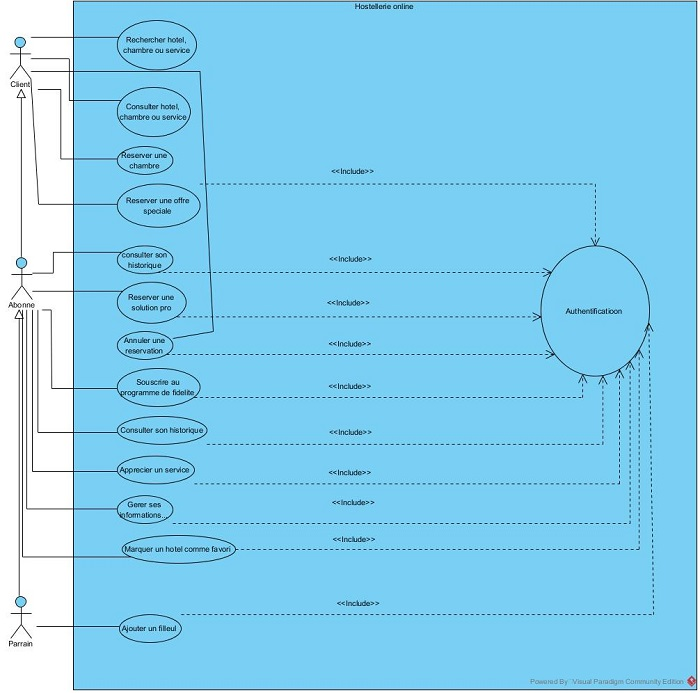
\includegraphics[scale=0.8]{images/diag_use_case1.jpg}
		\caption{schéma illustrant le diagramme de cas d’utilisation de la partie client}
		\label{synthese-cout-salarieg}
	\end{center}
\end{figure}

\cleardoublepage
\begin{figure}[h]
	\begin{center}
		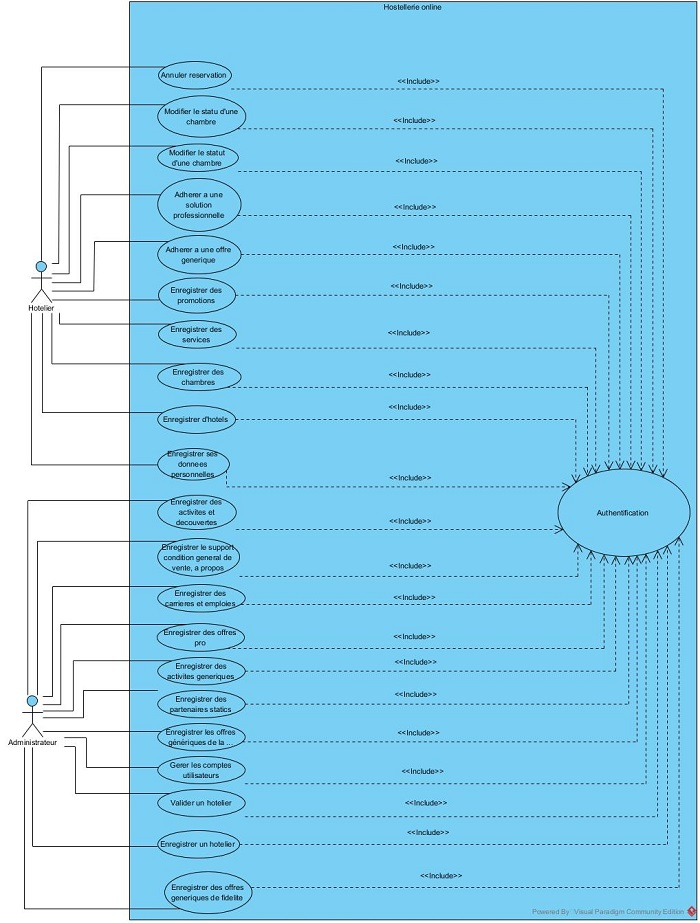
\includegraphics[scale=0.75]{images/diag_use_case2.jpg}
		\caption{schéma illustrant une partie du diagramme de cas d’utilisation partie administrateurs}
		\label{synthese-cout-salarieu}
	\end{center}
\end{figure}

\cleardoublepage
\subsection{DIAGRAMME DE SEQUENCE}
Le diagramme de séquence permet de montrer les interactions entre les acteurs et le système selon un ordre chronologique.

\begin{figure}[h]
	\begin{center}
		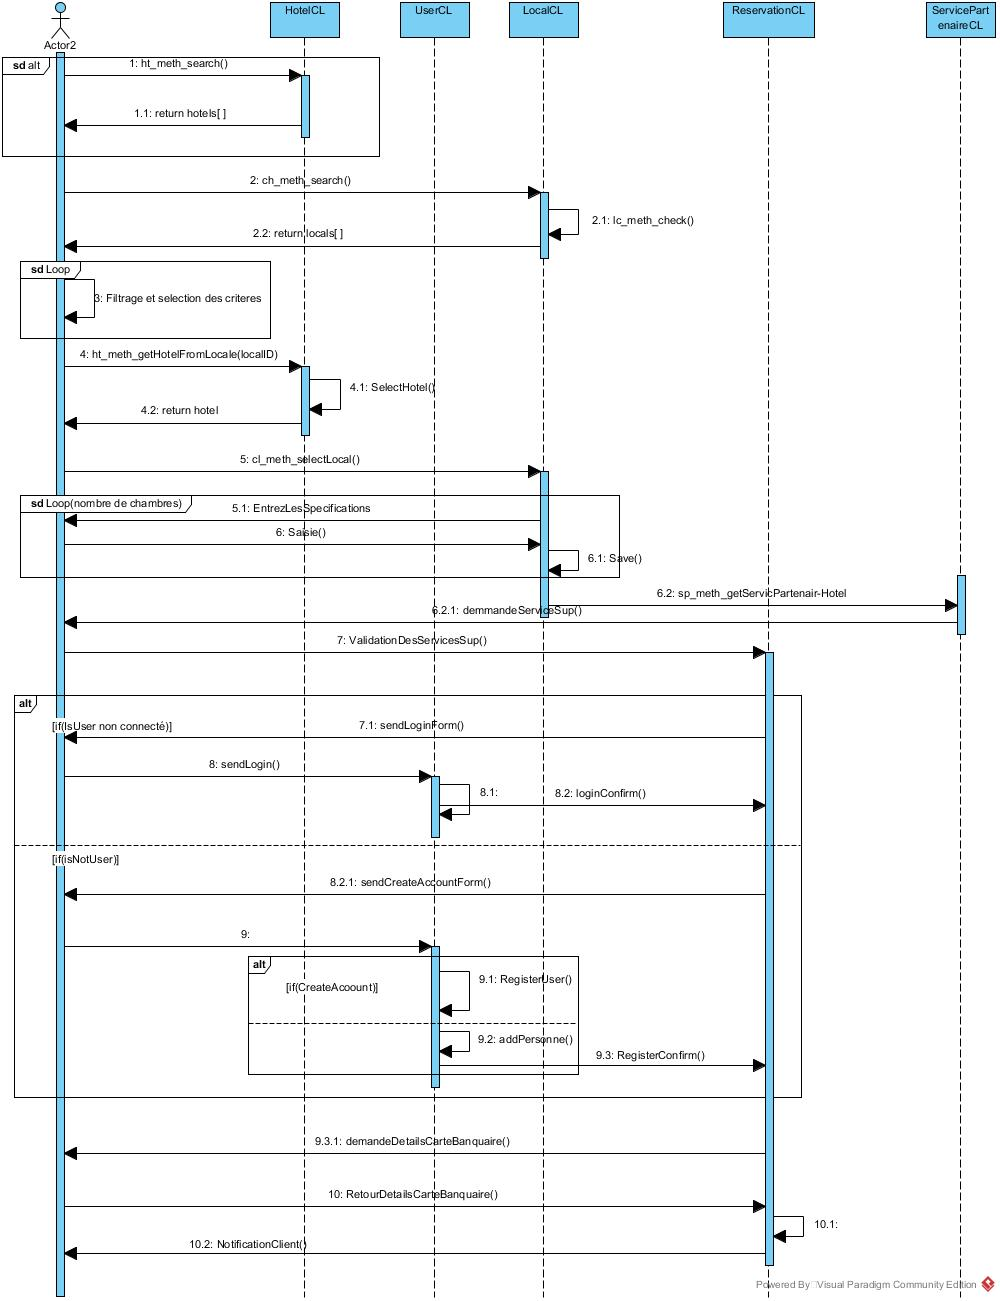
\includegraphics[scale=0.4]{images/Diagramme_de_sequence.jpg}
		\caption{Schéma illustrant le diagramme de séquence du cas RESERVATION}
		\label{synthese-cout-salariev}
	\end{center}
\end{figure}

\cleardoublepage
\subsection{DIAGRAMME DE CLASSE}
Le diagramme de classe est un schéma utilisé pour présenter les classes et les interfaces des systèmes ainsi que les différentes relations entre celles-ci.

\begin{figure}[h]
	\begin{center}
		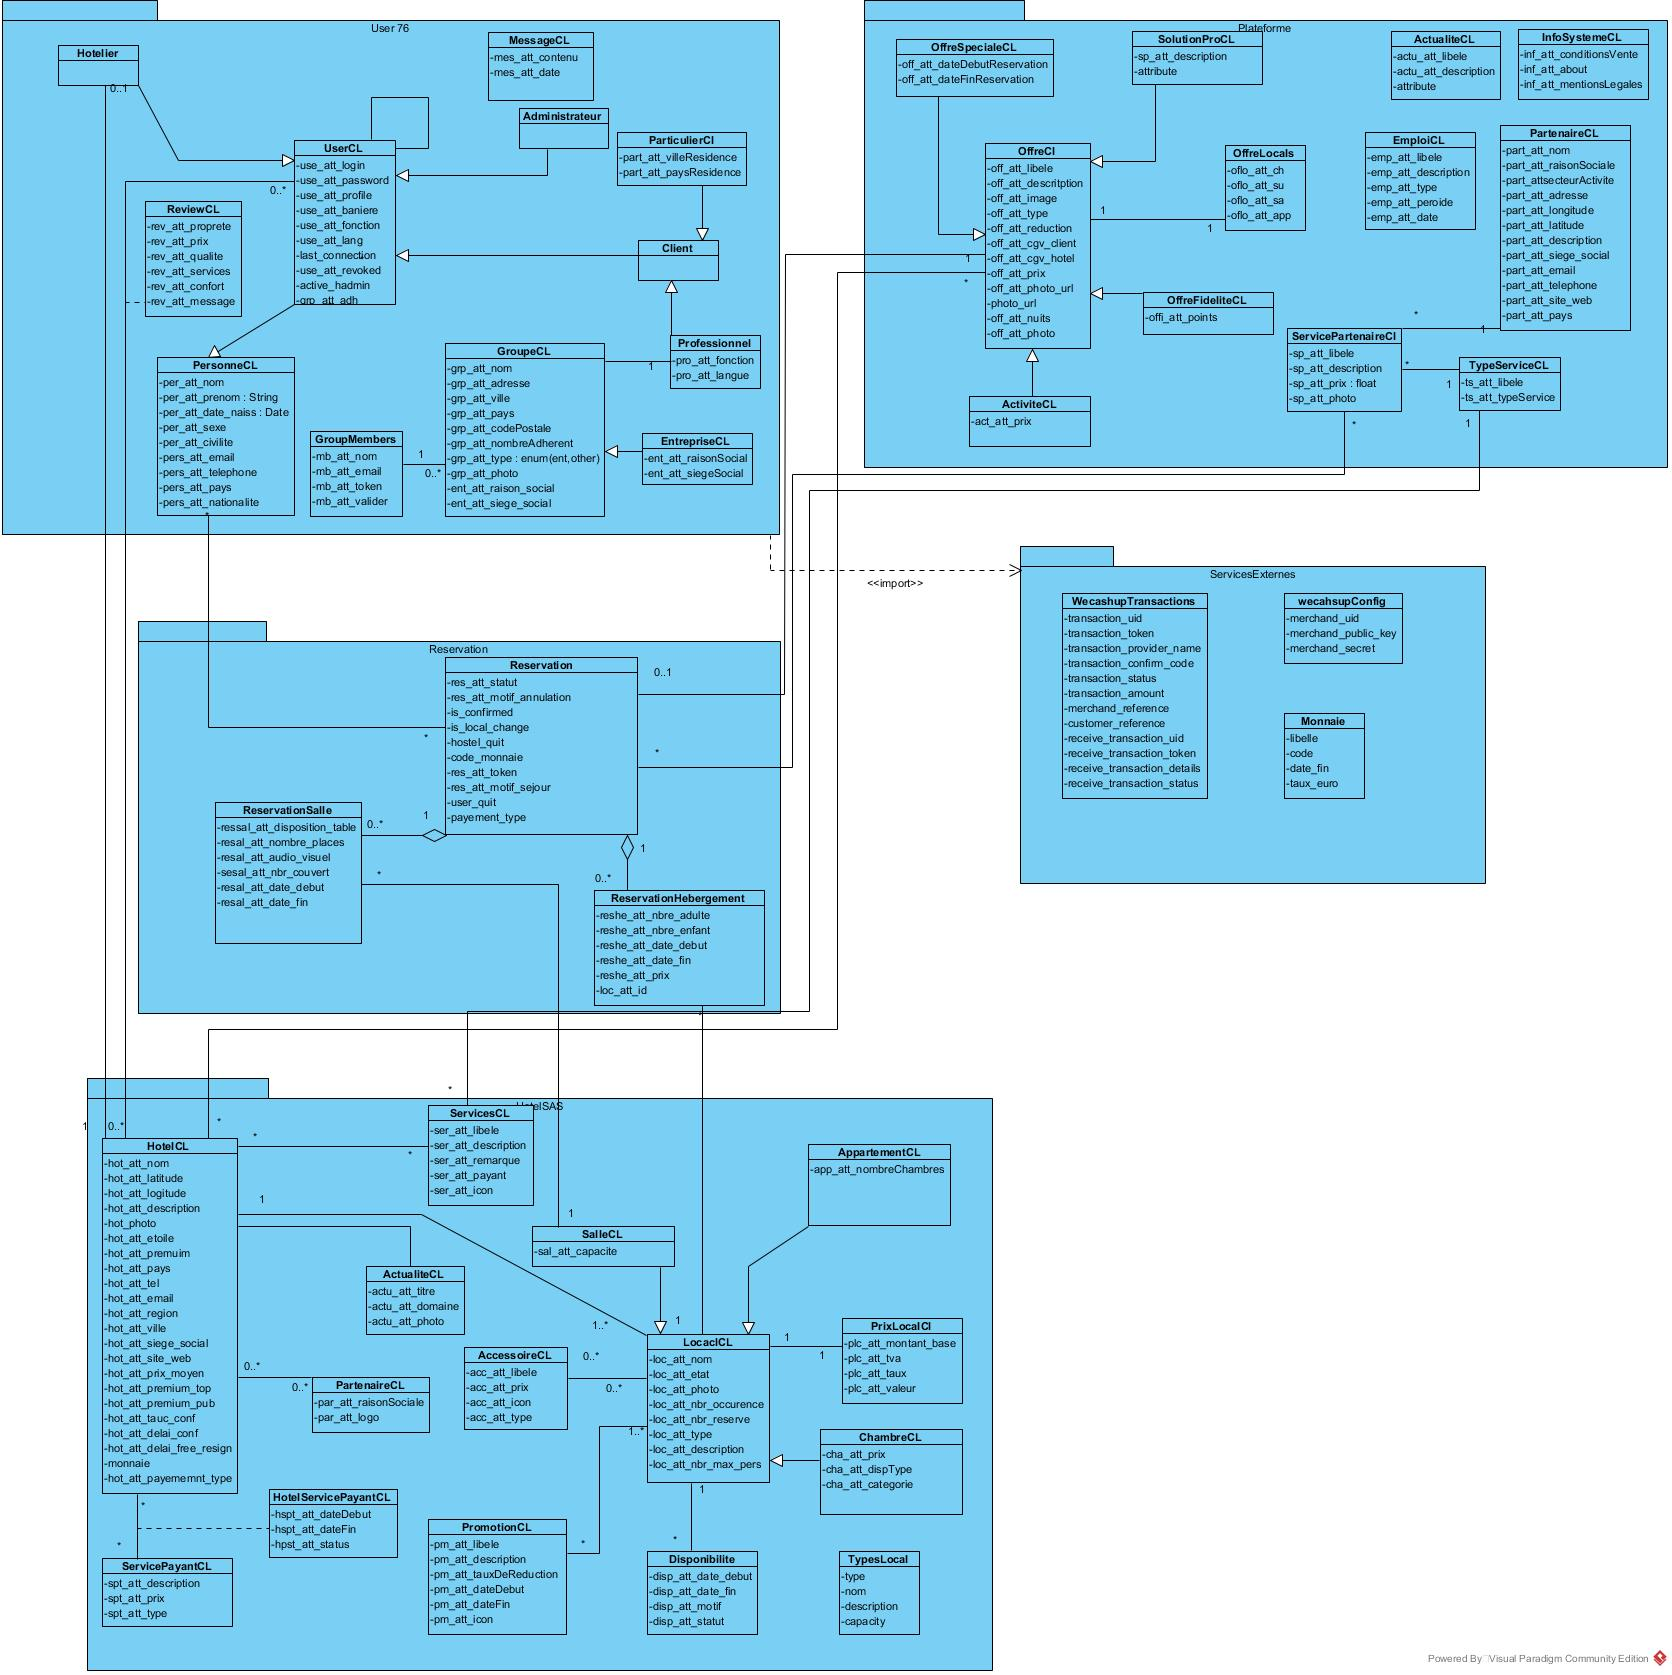
\includegraphics[scale=0.3]{images/diag_classe.jpg}
		\caption{schéma illustrant le diagramme de classe \(Agrandie en annexe\)}
		\label{synthese-cout-salariej}
	\end{center}
\end{figure}


\subsection{DIAGRAMME DE DÉPLOIEMENT}

Un diagramme de déploiement est une vue statique qui sert à représenter l'utilisation de l'infrastructure physique par le système et la manière dont les composants du système sont répartis ainsi que leurs relations entre eux.

\begin{figure}[h]
	\begin{center}
		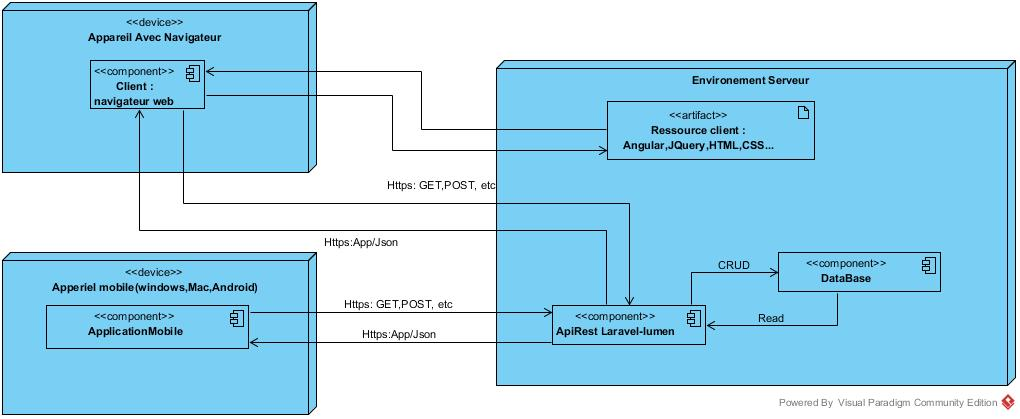
\includegraphics[scale=0.5]{images/Deployment_Diagram.jpg}
		\caption{schéma illustrant le diagramme de déploiement}
		\label{synthese-cout}
	\end{center}
\end{figure}

\section{CONCEPTION GENERALE}

\subsection{ARCHITECTURE}

 \textbf{ARCHITECTURE MATERIELLE}\\
 
L’implémentation de l’application impose une architecture 3-tiers dans laquelle celle-ci est le 2ième tiers encore appelé Middleware ; la base de données est le 3ème tiers et le client qui envoie une requête. Ce client est un navigateur web.

 \textbf{ARCHITECTURE LOGICIELLE}\\
 
L’architecture utilisée est le MVC (Modèle Vue Contrôleur) avec PHP et JAVA qui procure divers avantages comme la meilleure coordination de la division des tâches et la simplification de la maintenance aussi bien corrective qu’évolutive chacune des couches ayant un rôle précis. Le système de gestion de base de données utilisé est MySQL SERVER.

\subsection{OUTILS DE DEVELOPPEMENT}

 \textbf{LES OUTILS}\\
 
Les outils utilisés pour la réalisation de ce projet sont :
\begin{list}{•}{ }
\item \textbf{Visual Paradigme} : Analyse avec la méthode UML (diagramme de cas d’utilisation, de séquence, de classe, de déploiement).
\item \textbf{PHP Storm} : Environnement de développement intégré qui nous a permis d’écrire le code partie web pour concevoir cette application. 
\item \textbf{MySQL} : pour le stockage permanent des données.
\item \textbf{FileZilla} : client ftp pour le transfert de fichiers
\item \textbf{WAMP Server} : outil complet pour la simulation d’un environnement serveur en local.   
\item \textbf{1 and 1 }: Hébergement en ligne.
\end{list}

 \textbf{LES LANGAGES ET TECHNOLOGIES}
Les langages et technologies utilisés pour la réalisation de ce projet sont :
\begin{list}{•}{ }
\item HTML5/CSS3 : permet de structurer et formater les pages web de l’application.
\item AngularTS : Framework JavaScript contentent la partie client.
\item LARAVEL : Framework PHP permettant de développer les fonctionnalités côtés serveurs de l’application.
\item JAVASCRIPT : permet de faire les animations entre les différentes pages.
\end{list}
